\documentclass{standalone}
\usepackage{tikz}

\usetikzlibrary{calc,shadows,math}


\begin{document}

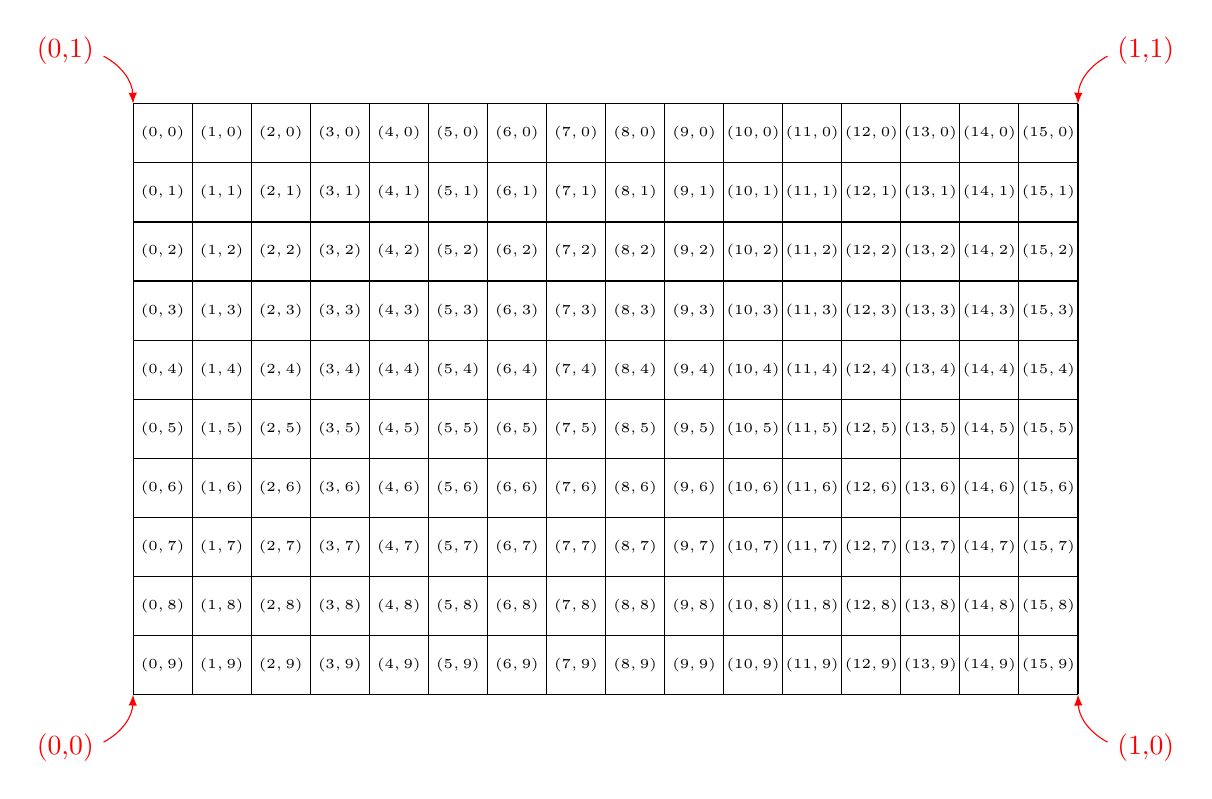
\begin{tikzpicture}
  \begin{scope}[scale=0.75]
    \draw[thin] (0,0) grid (16,10);
  
    \node[red,anchor=south east] (upper left) at (-0.5,10.5) {(0,1)};
    \draw[red,-latex] (upper left) to[bend left=30] (0,10);

    \node[red,anchor=south west] (upper right left) at (16.5,10.5) {(1,1)};
    \draw[red,-latex] (upper right left) to[bend right=30] (16,10);

    \node[red,anchor=north east] (lower left) at (-0.5,-0.5) {(0,0)};
    \draw[red,-latex] (lower left) to[bend right=30] (0,0);

    \node[red,anchor=north west] (lower right) at (16.5,-0.5) {(1,0)};
    \draw[red,-latex] (lower right) to[bend left=30] (16,0);

    \foreach[count=\i] \x in {0.5,...,15.5} {
      \foreach[count=\j] \y in {0.5,...,9.5} {
        \tikzmath{
          int \cx, \cy;
          \cx = \i - 1;
          \cy = 10 - \j;
        }
        \node[font=\tiny] at (\x,\y) {$(\cx, \cy)$};
      }
    }
  \end{scope}
\end{tikzpicture}

\end{document}